%%=============================================================================
%% Methodologie
%%=============================================================================

\chapter{\IfLanguageName{dutch}{Methodologie}{Methodology}}
\label{ch:methodologie}

%% TODO: Hoe ben je te werk gegaan? Verdeel je onderzoek in grote fasen, en
%% licht in elke fase toe welke stappen je gevolgd hebt. Verantwoord waarom je
%% op deze manier te werk gegaan bent. Je moet kunnen aantonen dat je de best
%% mogelijke manier toegepast hebt om een antwoord te vinden op de
%% onderzoeksvraag.

In hoofdstuk 2 is het onderzoek gestart met een literatuurstudie waarin besproken werd wat REST, JSON, gRPC en Protobufs exact zijn en hoe de interne architectuur van Fashion Society er uitziet.

In dit hoofdstuk gaat het onderzoek verder met een requirementanalyse en een plan van aanpak waarin beschreven wordt hoe de proof-of-concept tot stand komt.



\section{Requirementanalyse}
\label{sec:Requirementanalyse}

In deze analyse worden de functionele en niet-functionele vereisten opgelijst waaraan een alternatieve implementatie van de Discovery API moet voldoen.

Functionele requirements:
\begin{itemize}
    \item .NET Core 3.1 voor long-term support.
\end{itemize}

Niet-functionele requirements:


\section{Plan van aanpak}
\label{sec:Plan van aanpak}

\subsection{Opstellen van gRPC service in .NET Core 3.1 }
\label{subsec:Opstellen van gRPC service in .NET Core 3.1}
Uit de requirementanalyse kan afgeleid worden dat de service zal moeten draaien in .NET Core 3.1 en niet in .NET Core 5.0 omdat deze geen long-term support heeft van Microsoft.

Zodat gebruik gemaakt kan worden van de voordelen van gRPC zoals codegeneratie zal het project opgebouwd worden vanuit een grpc service project vanuit Visual Studio zelf, dit project bevat de Grpc.AspNetCore package die alles gRPC gerelateerd afhandelt.

Voor de logica in de twee endpoints GetService en GetServiceUrl die respectievelijk een service object en een service url ophalen zal code gerecupereerd worden van de reeds bestaande Discovery API.

De reeds bestaande Discovery API maakt gebruik van het repository patroon voor het ophalen en verwerken van data uit een SQL database in de gRPC service zal dit patroon wegvallen en zal de databasecontext rechtstreeks in de Service geïnjecteerd worden. Uit een verdere analyse van de bestaande code kan er ook geconcludeerd worden dat beide methoden gebruik maken van éénzelfde Get methode in de repository, deze wordt een private methode in de Service die zal worden aangesproken door beide endpoints.

Het protobestand “services.proto” waaruit de bijhorende modellen worden gegenereerd bevat de 2 rpc methodes GetService en GetServiceUrl, beiden hebben deze een input parameter van het messagetype “ServiceName” met als veld een string “name”.
De GetService methode zal een message van het type “ServiceObject” teruggeven, deze bevat de “name”, “address”, “port”, “addNameToUrl” en “hasSwaggedDoc” velden. Deze velden zijn licht afwijkend van het reeds bestaande Model in de Discovery API maar is in samenspraak met mijn co-promotor.
Tot slot is er de GetServiceUrl methode, deze geeft een message van het type “ServiceUrl” terug dewelke een enkel veld bevat zijnde “url”.

In figuur \ref{fig:ProtoPoC} is het gebruikte protobestand te zien.

\begin{figure}[H]
    \centering
    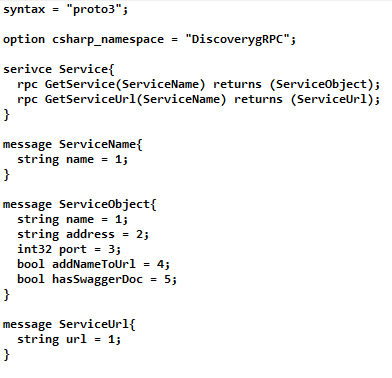
\includegraphics[scale=0.75]{ProtoPoC}
    \caption[Proof-Of-Concept protobestand]{Het gebruikte protobestand}
    \label{fig:ProtoPoC}
\end{figure}

\subsection{Client applicaties voor REST en gRPC}
\label{subsec:Client applicaties voor REST en gRPC}

Om de snelheid van beide implementaties te testen moeten de services worden aangesproken van een client. Hiervoor worden twee identieke implmentaties gebruikt in twee Console applicaties (.NET Core). De enige verschillen tussen de twee applicaties zijn de aangesproken endpoints. Deze applicaties zullen aan de hand van een lijst van vier servicenamen calls doen naar de service. Er is voor vier servicenamen gekozen zodanig dat er rekening wordt gehouden met eventuele verschillen in het ophalen van de verschillende data.

Tijdens het gehele proces zullen twee timers lopen, een overlappende timer die de totale tijd van de calls zal opnemen en een timer die per 100 calls de tijd in miliseconden zal wegschrijven naar een lijst die na afloop zal worden geëxporteerd naar een bestand.

\subsection{Het verloop van het onderzoek}
\label{subsec:Het verloop van het onderzoek}

Het onderzoek wordt uitgevoerd in drie categorieën, een kleine en grote payload voor het resultaat van parallele requests en een request loop van tienduizend requests voor een gewogen resultaat voor één request te berekenen. In de kleine payload zullen er in totaal vierduizend calls gemaakt worden, elke servicenaam zal tien keer parallel gebruikt worden om vervolgens honderd requests te versturen. In de grote payload zullen er veertigduizend calls gemaakt worden en hier zal elke servicenaam honderd keer parallel gebruikt worden om vervolgens honderd requests te versturen.

De kleine en grote payload zullen vier keer uitgevoerd worden om tot een concreet resultaat te bekomen.

Het CPU gebruik zal manueel in de gaten gehouden worden maar zal in samenspraak met de co-promotor niet in acht genomen worden in de resultaten omdat er geen accurate manier beschikbaar is om het CPU gebruik op de server te registreren.

